%!TEX root = ../thesis.tex
%*******************************************************************************
%****************************** Fifth Chapter **********************************
%*******************************************************************************
\chapter{Ballistic Deposition on Square Lattice}

% **************************** Define Graphics Path **************************
\ifpdf
    \graphicspath{{Chapter5/Figs/}{Chapter5/Figs/L0/}{Chapter5/Figs/L1/}{Chapter5/Figs/L2/}}
\else
    \graphicspath{{Chapter5/Figs/}{Chapter5/Figs/L0/}{Chapter5/Figs/L1/}{Chapter5/Figs/L2/}}
\fi

Imagine a spherical shaped object, say marble, is thrown on top of a 2D square lattice structure. First possible scenario is that the marble will be deposited in the first encountered site in the lattice . Now if the first encountered site is not empty, the possible scenario is that the marble will go in any of the four direction, $+x$, $-x$, $+y$ or $-y$, assuming no other direction in between is allowed in the lattice.  Now if the first neighbor is not empty then the marble will continue to go on in the previously selected direction and choose the next neighbor. This is the main theme of this thesis.\\
In our experiment, we occupy a randomly chosen site if it is empty else we select one of its four neighbor to occupy if it is empty else select next neighbor in that direction and occupy that site if it is empty else ignore current iteration and choose another site randomly. This process is repeated until there is no empty site in the lattice. We call this process the ballistic deposition on the square lattice. We introduce 1st and 2nd nearest neighbor interaction in this way.
\section{Building The Structure}
\section{Percolation Algorithm}
\begin{enumerate}
	\item take a square lattice of length $L$.
	\item choose a site randomly
	\item if the chosen site is empty then occupy it else choose one of the four neighbor randomly
	\item if the chosen neighbor is empty then occupy it else choose second nearest neighbor in that direction
	\item if the second nearest neighbor is empty then occupy the site else ignore this step
\end{enumerate}
\section{Finite Size Scaling in Percolation Theory}
\section{Finding Numerical Values}
	\subsection{Critical occupation probability, $p_c$}
	When we occupy sites of the square lattice, initially, there are only cluster of size 1. As we keep occupying different size of clusters starts to appear. At a certain point a special cluster appears which spans the entire lattice. We call this cluster the \textit{Spanning Cluster}. It should be noted that the spanning cluster is a special property of the lattice and the appearance of the spanning cluster is the result of phase transition. At the point where the spanning cluster first appears is called the critical point and denoted by $p_c$, meaning the occupation probability at the critical point. The figure \ref{finding-pc} shows the graph of the spanning probability, $w(p,L)$, versus the occupation probability $p$ for different interactions ($L0, L1, L2$) for different lengths. We have found that $p_c$ is $0.5927, 0.5782, 0.5701$ for $L0, L1, L2$ respectively.Thus for long range interaction $p_c$ is smaller than for short range interaction. 
		\begin{figure}
			\begin{subfigure}{0.329\textwidth}
				\centering
				\includegraphics[width=\linewidth]{{{sq_lattice_site_percolation_periodic_-occupation_probability-pc0.5927}}}
				\caption{L0}
			\end{subfigure}
			\begin{subfigure}{0.329\textwidth}
				\centering
				\includegraphics[width=\linewidth]{{{sq_lattice_site_percolation_ballistic_deposition_L1_periodic_-occupation_probability-pc0.5782}}}
				\caption{L1}
			\end{subfigure}
			\begin{subfigure}{0.329\textwidth}
				\centering
				\includegraphics[width=\linewidth]{{{sq_lattice_site_percolation_ballistic_deposition_L2_periodic_-occupation_probability-pc0.5701}}}
			\caption{L2}
			\end{subfigure}
			\caption{Spanning Probability, $w(p,L)$ vs Occupation Probability, $p$}
			\label{finding-pc}
		\end{figure}
	The quantity $w(p, L)$ is called the spanning probability in a non periodic case and wrapping probability in a periodic case.
	The question is how do we find the wrapping probability, given that we have a list of $p_c$ for different length. Note that for a certain length $L$, in each realization the $p_c$ is not exact value, instead it is a range of values that contains the $p_c$. For example, say we have a lattice of length $200$ and for that we will have different $p_c$ at each realization. After an infinite number of experimentation we will have to take an average and that will give the exact value of $p_c$. But since it is practically impossible, we can find $p_{c_{avg}}$ for different lattice size then from the graph we can extrapolate the exact value of $p_c$ for infinite lattice. Here $p_{c_{avg}}$ is calculated from a finite set of $p_c$ for a certain length. This process is not good enough. Since it requires  $p_{c_{avg}}$'s for a number of lattice size which is very costly to obtain. But from the data, list of $p_c$'s for different length, we can find the cumulative frequency distribution. It is astonishing  that for all length the wrapping probability coincide at a specific point. This implies that if we could have an infinite system, the wrapping probability for that system would have gone through this same point. This means we got our critical point, $p_c$, as the intersection of the $w(p,L)$ for different lengths.
	\subsection{Spanning Probability and finding $1/\nu$} \label{section:spanning-probability-and-one-by-nu}
	From the figure \ref{finding-pc} we can see that, as we increase the length of the lattice the wrapping probability $w(p,L)$ moves closer and closer to the critical point. And if we draw a horizontal line at a certain height, say $y=0.1$, and find the intersection of this line with $w(p,L)$ for each length  and note the $p$ and if we plot $\log(L)$ vs $\log(p-p_c)$ we get the slope $1/\nu$. If we now use the finite size scaling (FSS) hypothesis
	\begin{equation}
		w = (p-p_c) L^{1/\nu}
	\end{equation}
	we get a very good data collapse for $L0,L1,L2$ and got $1/\nu$ as $0.75, 0.736, 0.721$ respectively which is shown in figure \ref{spanning-probability-data-collapse}. That is they are self-similar \ref{label}.
		\begin{figure}
			\begin{subfigure}{0.329\textwidth}
				\centering
				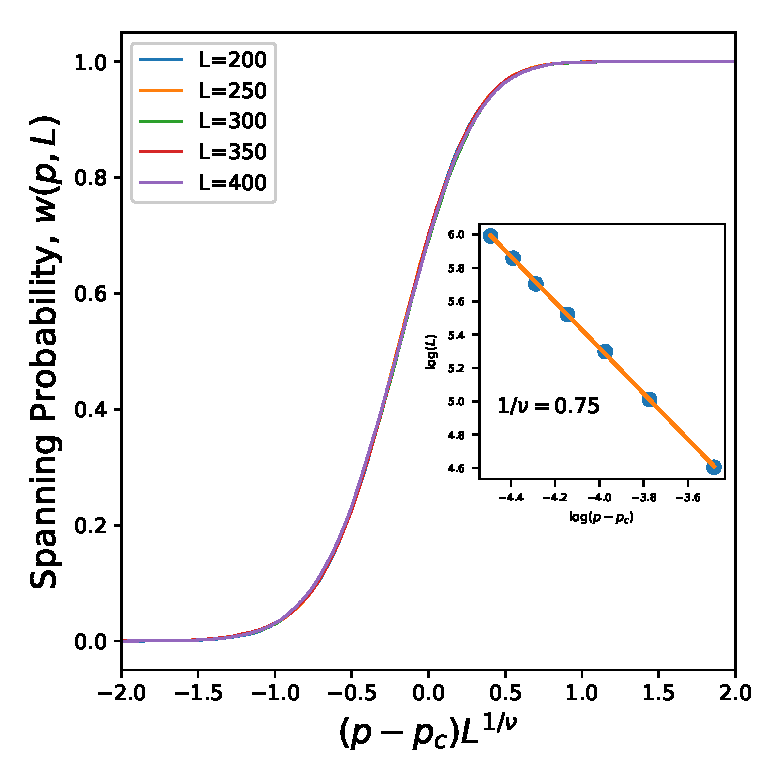
\includegraphics[width=\linewidth]{{{L0/sq_lattice_site_percolation_periodic_-occupation_probability-data_collapse-pc0.5927-ex0.7500}}}
				\caption{L0}
			\end{subfigure}
			\begin{subfigure}{0.329\textwidth}
				\centering
				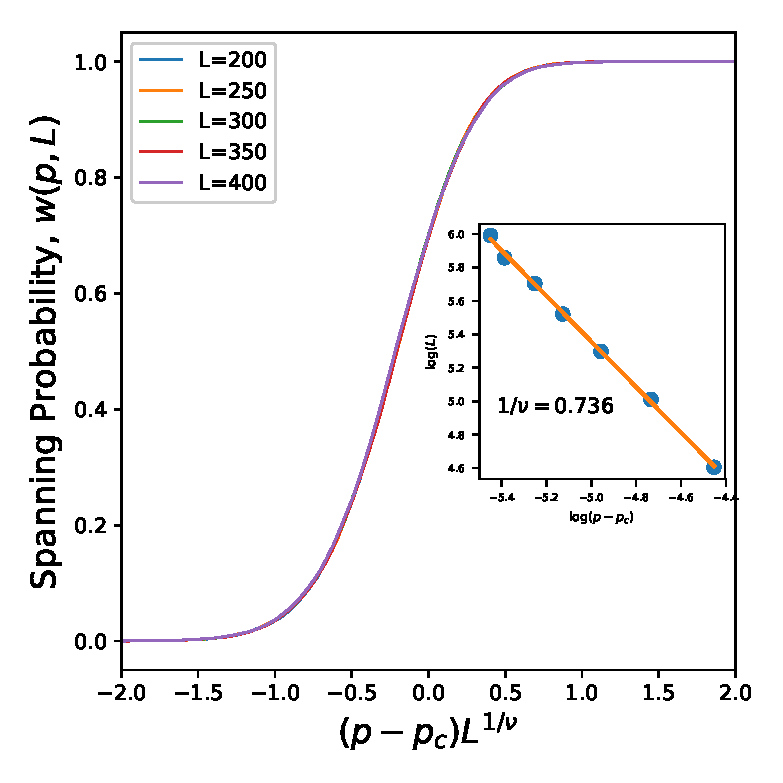
\includegraphics[width=\linewidth]{{{L1/sq_lattice_site_percolation_ballistic_deposition_L1_periodic_-occupation_probability-data_collapse-pc0.5782-ex0.7360}}}
				\caption{L1}
			\end{subfigure}
			\begin{subfigure}{0.329\textwidth}
				\centering
				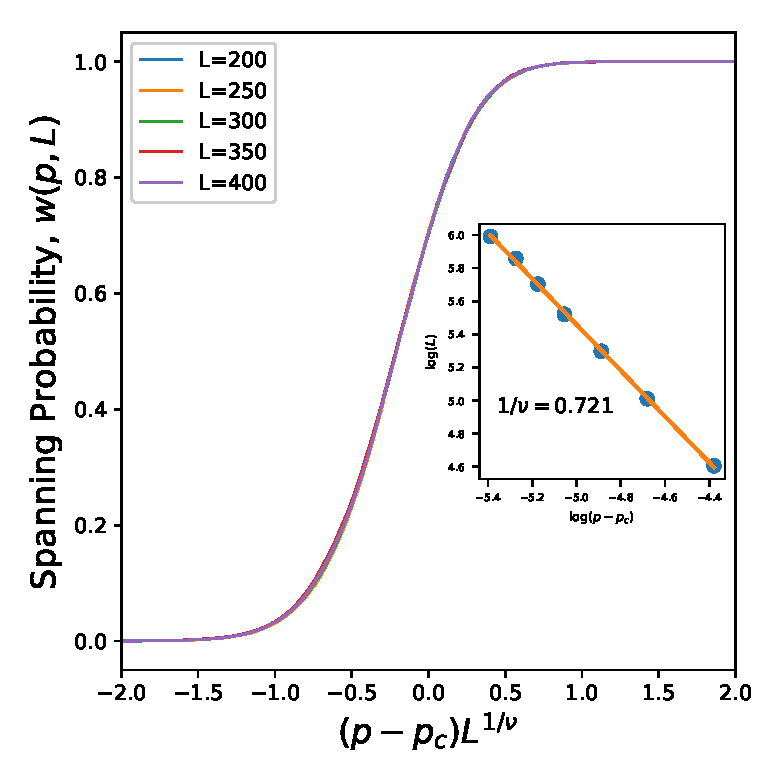
\includegraphics[width=\linewidth]{{{L2/sq_lattice_site_percolation_ballistic_deposition_L2_periodic_-occupation_probability-data_collapse-pc0.5701-ex0.7210}}}
				\caption{L2}
			\end{subfigure}
			\caption{$w(p,L)$ vs $(p-p_c) L^{1/\nu}$}
			\label{spanning-probability-data-collapse}
		\end{figure}
	
	\subsection{Entropy, Specific Heat and finding $\alpha$}
		For any phase transition model the entropy is crucial. In percolation theory we use Shannon Entropy \cite{shanon_entropy}. Using the definition \ref{label} we get the figure \ref{fig:entropy}
		\begin{figure}
			\begin{subfigure}{0.329\textwidth}
				\centering
				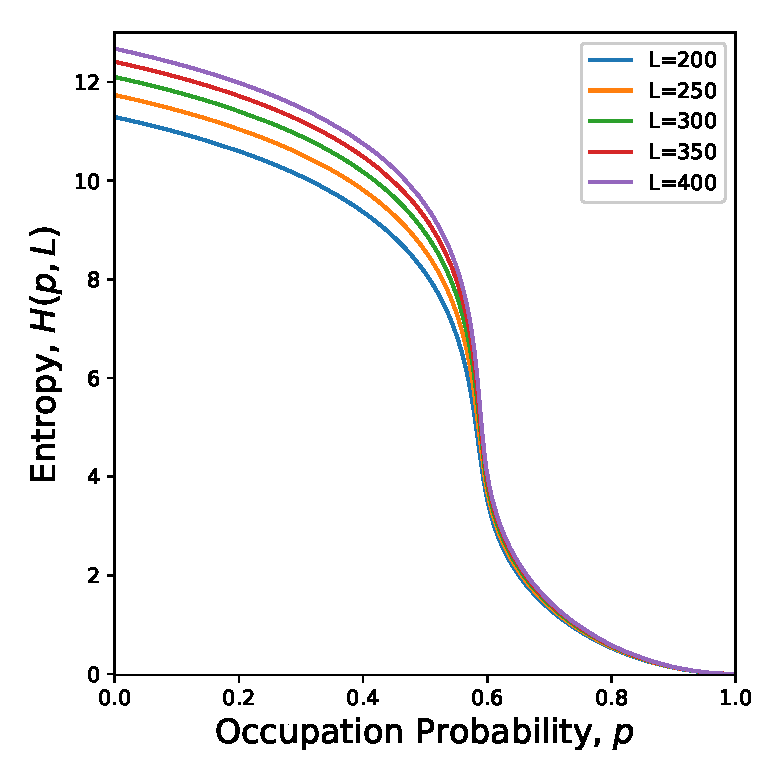
\includegraphics[width=\linewidth]{{{L0/sq_lattice_site_percolation_periodic_-entropy}}}
				\caption{L0}
			\end{subfigure}
			\begin{subfigure}{0.329\textwidth}
				\centering
				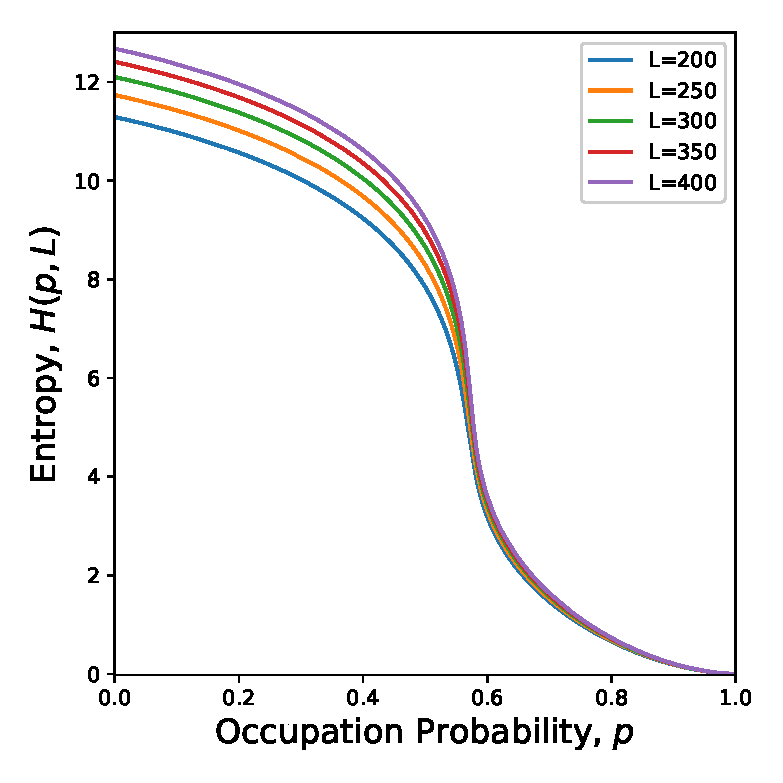
\includegraphics[width=\linewidth]{{{L1/sq_lattice_site_percolation_ballistic_deposition_L1_periodic_-entropy}}}
				\caption{L1}
			\end{subfigure}
			\begin{subfigure}{0.329\textwidth}
				\centering
				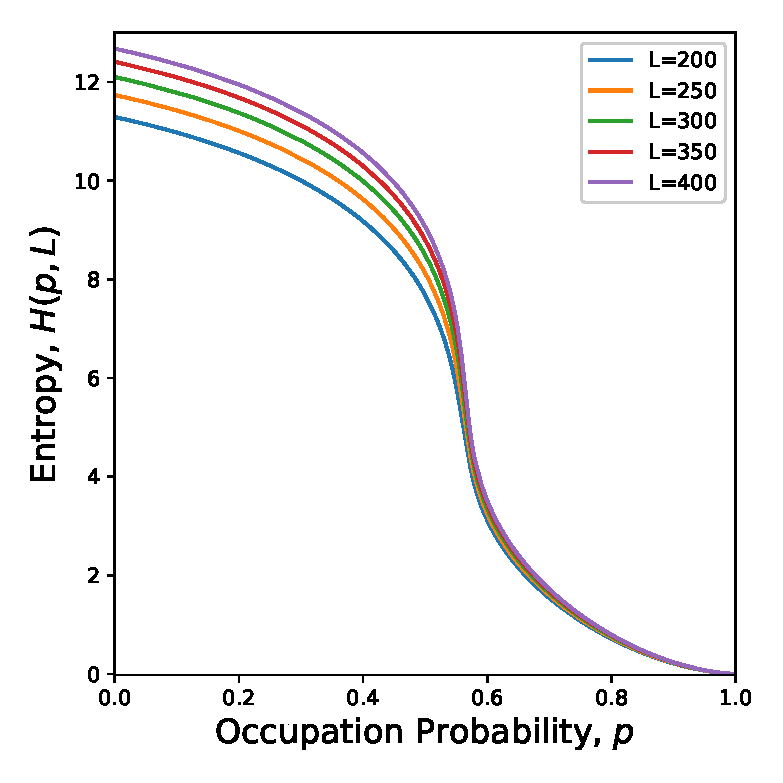
\includegraphics[width=\linewidth]{{{L2/sq_lattice_site_percolation_ballistic_deposition_L2_periodic_-entropy}}}
				\caption{L2}
			\end{subfigure}
			\caption{Entropy, $H(p,L)$ vs Occupation Probability, $p$}
			\label{fig:entropy}
		\end{figure}
	And since the specific heat $C(p,L)$ is nothing but the derivative of entropy, by simply differentiating entropy we get the specific heat (although we need to perform convolution\ref{} in order to get a smooth curve) shown in figure \ref{fig:specific-heat-graph}.
		\begin{figure}
			\begin{subfigure}{0.329\textwidth}
				\centering
				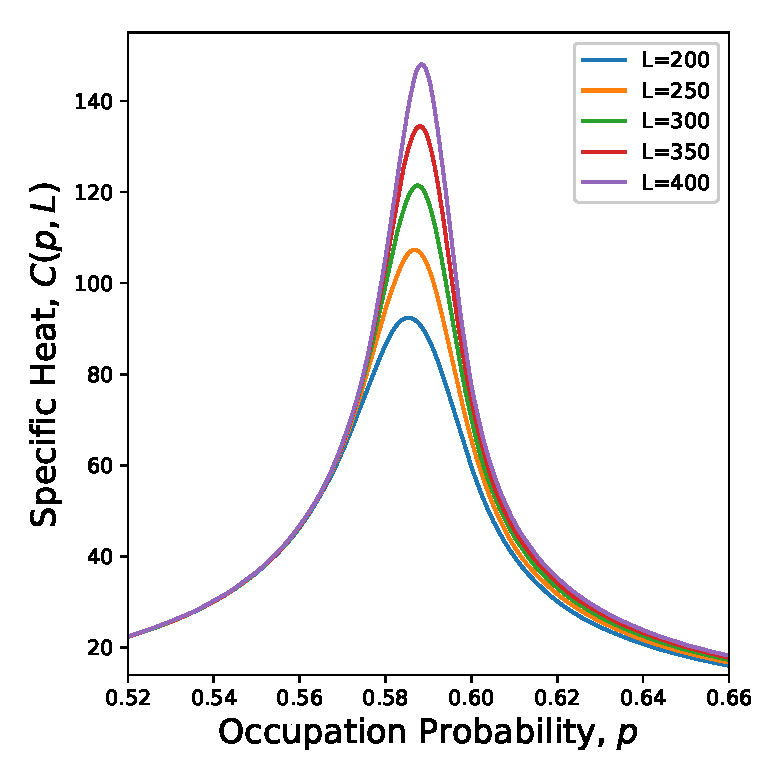
\includegraphics[width=\linewidth]{{{L0/sq_lattice_site_percolation_periodic__specific_heat-pc0.5927}}}
				\caption{L0}
			\end{subfigure}
			\begin{subfigure}{0.329\textwidth}
				\centering
				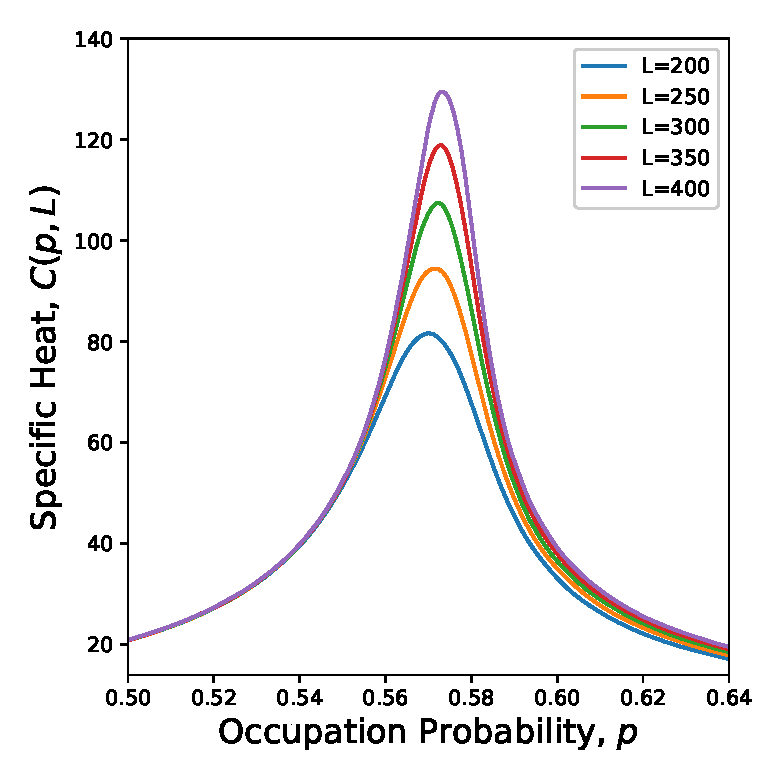
\includegraphics[width=\linewidth]{{{L1/sq_lattice_site_percolation_ballistic_deposition_L1_periodic__specific_heat-pc0.5782}}}
				\caption{L1}
			\end{subfigure}
			\begin{subfigure}{0.329\textwidth}
				\centering
				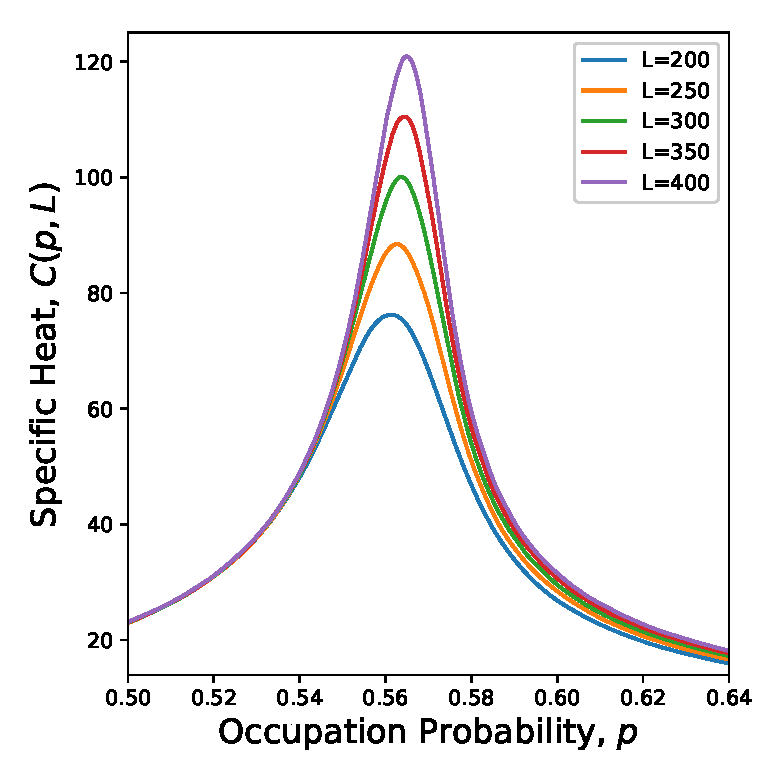
\includegraphics[width=\linewidth]{{{L2/sq_lattice_site_percolation_ballistic_deposition_L2_periodic__specific_heat-pc0.5701}}}
				\caption{L2}
			\end{subfigure}
			\caption{Specific Heat, $C(p,L)$ vs Occupation Probability, $p$}
			\label{fig:specific-heat-graph}
		\end{figure}
		From specific heat we can find the exponent $\alpha$. To do this first we need to scale the $x$-values of the specific heat data using the exponent $1/\nu$ obtained from \ref{section:spanning-probability-and-one-by-nu} and get the graph as in figure \ref{fig:specific-heat-x-scaled-graph}. From this graph we will not the height of each line and call it $C_h$. Since each line corresponds to a specific length $L$ we can plot $\log(C_h)$ versus $\log(L)$ and the absolute value of the graph will give $\alpha/\nu$ and from that we can find the exponent $\alpha$ simply by dividing $\alpha/\nu$ by $1/\nu$. We get $\alpha$ values $0.906,0.911,0.919$ for $L0,L1,L2$ correspondingly. and using this value we can apply FSS hypothesis to get data collapse.
		\begin{figure}
			\begin{subfigure}{0.329\textwidth}
				\centering
				\includegraphics[width=\linewidth]{{{sq_lattice_site_percolation_periodic__specific_heat-x-scaled-pc0.5927_alpha_0.6799_nu_0.750}}}
				\caption{L0}
			\end{subfigure}
			\begin{subfigure}{0.329\textwidth}
				\centering
				\includegraphics[width=\linewidth]{{{sq_lattice_site_percolation_ballistic_deposition_L1_periodic__specific_heat-x-scaled-pc0.5782_alpha_0.6712_nu_0.736}}}
				\caption{L1}
			\end{subfigure}
			\begin{subfigure}{0.329\textwidth}
				\centering
				\includegraphics[width=\linewidth]{{{sq_lattice_site_percolation_ballistic_deposition_L2_periodic__specific_heat-x-scaled-pc0.5701_alpha_0.6631_nu_0.721}}}
				\caption{L2}
			\end{subfigure}
			\label{fig:specific-heat-x-scaled-graph}
			\caption{$C(p,L)$ vs $(p-p_c) L^{1/\nu}$}
		\end{figure}
	If we plot $C L^{-\alpha/\nu}$ vs $(p-p_c)L^{1/\nu}$ we get perfect data collapse for $L0,L1,L2$ and it is shown in figure \ref{fig:specific-heat-data-collapse-graph}
		\begin{figure}
			\begin{subfigure}{0.329\textwidth}
				\centering
				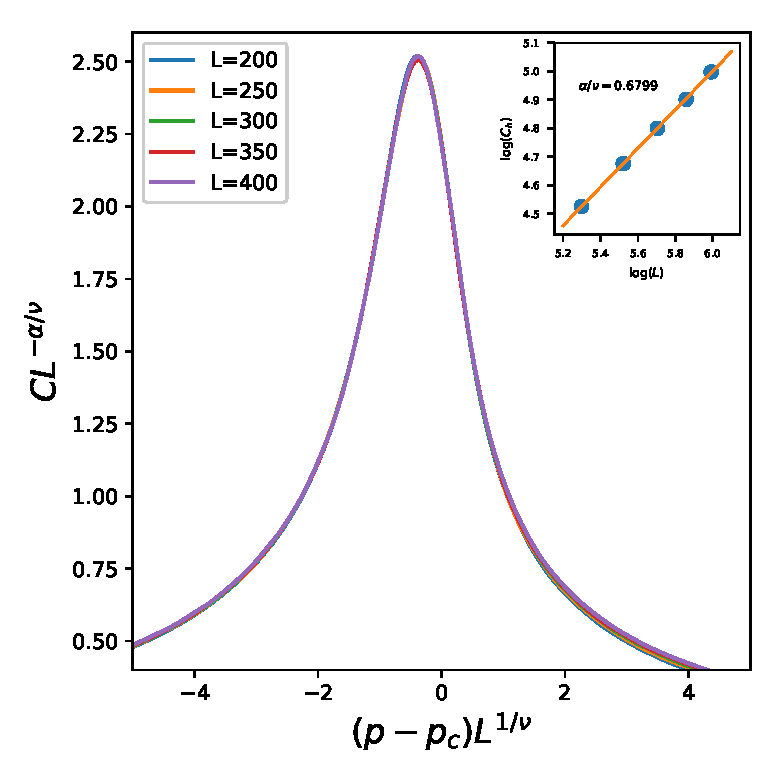
\includegraphics[width=\linewidth]{{{L0/sq_lattice_site_percolation_periodic__specific_heat-data_collapse-pc0.5927_alpha_0.6799_nu_0.750}}}
				\caption{L0}
			\end{subfigure}
			\begin{subfigure}{0.329\textwidth}
				\centering
				\includegraphics[width=\linewidth]{{{sq_lattice_site_percolation_ballistic_deposition_L1_periodic__specific_heat-data_collapse-pc0.5782_alpha_0.6712_nu_0.736-with}}}
				\caption{L1}
			\end{subfigure}
			\begin{subfigure}{0.329\textwidth}
				\centering
				\includegraphics[width=\linewidth]{{{sq_lattice_site_percolation_ballistic_deposition_L2_periodic__specific_heat-data_collapse-pc0.5701_alpha_0.6712_nu_0.721-with}}}
				\caption{L2}
			\end{subfigure}
			\caption{$C L^{-\alpha/\nu}$ vs $(p-p_c) L^{1/\nu}$}
			\label{fig:specific-heat-data-collapse-graph}
		\end{figure}
	\subsection{Order Parameter and finding $\beta$}
		Order parameter, also knows as the percolation strength, is ,along with entropy, an important quantity in the study of phase transition. It is denoted as $P(p,L)$. Using the definition \ref{def:order-parameter-2} we obtain the order parameter for our system and it is shown in the figure \ref{fig:order-parameter}. Since using spanning cluster and the largest cluster gives the same exponent, it really does not matter which one we use. But in our case there is a boundary of the system, which we define as periodic. Hence using spanning cluster is appropriate.
		\begin{figure}
			\begin{subfigure}{0.329\textwidth}
				\centering
				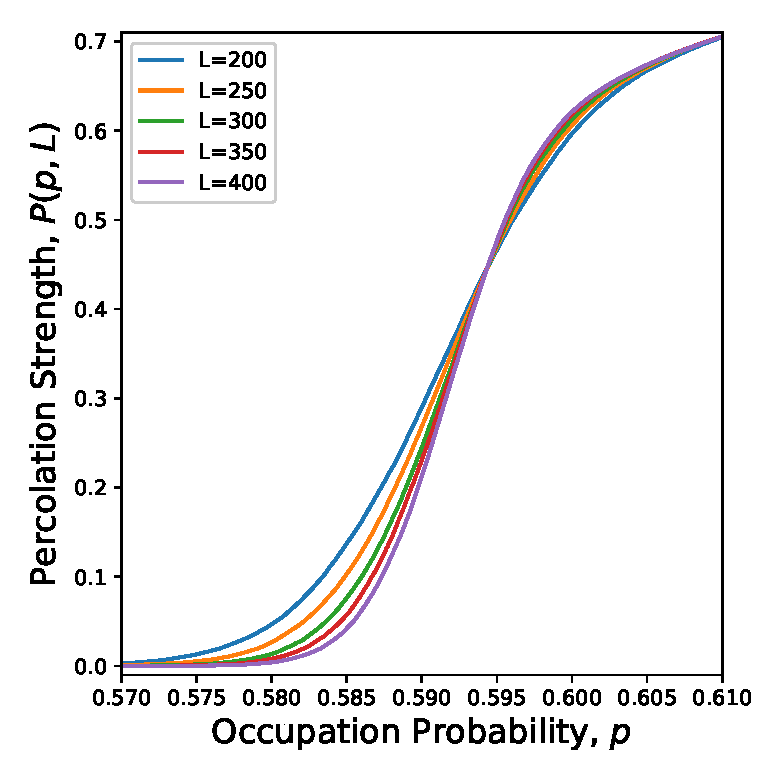
\includegraphics[width=\linewidth]{{{L0/sq_lattice_site_percolation_periodic_-spanning-_order_parameter-pc0.5927}}}
				\caption{L0}
			\end{subfigure}
			\begin{subfigure}{0.329\textwidth}
				\centering
				\includegraphics[width=\linewidth]{{{sq_lattice_site_percolation_ballistic_deposition_L1_periodic_-spanning-_order_parameter-pc0.5782}}}
				\caption{L1}
			\end{subfigure}
			\begin{subfigure}{0.329\textwidth}
				\centering
				\includegraphics[width=\linewidth]{{{sq_lattice_site_percolation_ballistic_deposition_L2_periodic_-spanning-_order_parameter-pc0.5701}}}
				\caption{L2}
			\end{subfigure}
			\caption{Order Parameter, $P(p,L)$ vs Occupation Probability, $p$}
			\label{fig:order-parameter}
		\end{figure}
		Using the exponent $1/\nu$ obtained in section \ref{section:spanning-probability-and-one-by-nu} we scale the $x$-values as $(p-p_c)L^{1/\nu}$ and get the following figure \ref{fig:order-parameter-x-scaled}.
		\begin{figure}
			\begin{subfigure}{0.329\textwidth}
				\centering
				\includegraphics[width=\linewidth]{{{sq_lattice_site_percolation_periodic_-spanning-_order_parameter-x-scaled-pc0.5927}}}
				\caption{L0}
			\end{subfigure}
			\begin{subfigure}{0.329\textwidth}
				\centering
				\includegraphics[width=\linewidth]{{{sq_lattice_site_percolation_ballistic_deposition_L1_periodic_-spanning-_order_parameter-x-scaled-pc0.5782}}}
				\caption{L1}
			\end{subfigure}
			\begin{subfigure}{0.329\textwidth}
				\centering
				\includegraphics[width=\linewidth]{{{sq_lattice_site_percolation_ballistic_deposition_L2_periodic_-spanning-_order_parameter-x-scaled-pc0.5701}}}
				\caption{L2}
			\end{subfigure}
			\caption{Order Parameter, $P(p,L)$ vs Occupation Probability, $p$}
			\label{fig:order-parameter-x-scaled}
			\caption{$P(p,L)$ vs $(p-p_c) L ^{1/\nu}$}
		\end{figure}
 	    Then in figure \ref{fig:order-parameter-x-scaled} we draw a vertical line where there are several horizontal lines. We measure the height of the lines and call it $P_h$ and after plotting $\log(P_h)$ vs $\log(L)$ (inset of figure \ref{fig:order-parameter-data-collapse})we get the exponent $\beta/\nu$ from it's slope and obtain exponent $\beta$ by dividing $\beta/\nu$ by $1/\nu$.
 	    Using the FSS hypothesis \ref{label} we plot $PL^{\beta/\nu}$ versus $(p-p_c)L^1/\nu$ and get a good data collapse which is shown in figure \ref{fig:order-parameter-data-collapse}.
		\begin{figure}
			\begin{subfigure}{0.329\textwidth}
				\centering
				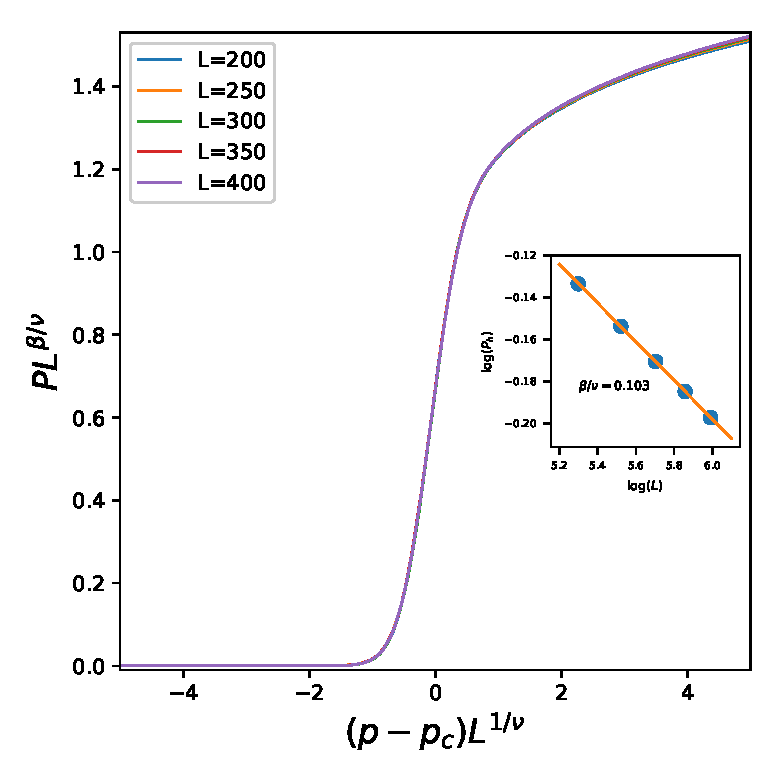
\includegraphics[width=\linewidth]{{{L0/sq_lattice_site_percolation_periodic_-spanning-_order_parameter-data_collapse-pc0.5927_beta_0.103_nu_0.750}}}
				\caption{L0}
			\end{subfigure}
			\begin{subfigure}{0.329\textwidth}
				\centering
				\includegraphics[width=\linewidth]{{{sq_lattice_site_percolation_ballistic_deposition_L1_periodic_-spanning-_order_parameter-data_collapse-pc0.5782_beta_0.103_nu_0.736}}}
				\caption{L1}
			\end{subfigure}
			\begin{subfigure}{0.329\textwidth}
				\centering
				\includegraphics[width=\linewidth]{{{sq_lattice_site_percolation_ballistic_deposition_L2_periodic_-spanning-_order_parameter-data_collapse-pc0.5701_beta_0.098_nu_0.721}}}
				\caption{L2}
			\end{subfigure}
			\caption{$P L^{\beta/\nu}$ vs $(p-p_c) L ^{1/\nu}$}
			\label{fig:order-parameter-data-collapse}
		\end{figure}
	\subsection{Susceptibility and finding $\gamma$}
	Susceptibility is defined as the derivative of the order parameter $P(p,L)$ with respect to the control parameter $p$,i.e., $\chi = \frac{dP}{dp}$. Using this definition we obtain the graph of susceptibility \ref{fig:susceptibility}. And if we scale the $x$ values and plot $\chi$ vs $(p-p_c)L^{1/\nu}$ we get all the peak point aligned (figure \ref{fig:susceptibility-x-scaled}). Note that the value of $1/\nu$ is known from section \ref{section:spanning-probability-and-one-by-nu}. Then we take the reading of the height of each line and call it $\chi_h$. Since each line represents a different lattice size, plotting $\log(\chi_h)$ vs $\log(L)$ gives the slope $\gamma/\nu$. And using the FSS hypothesis we plot $\chi L^{-\gamma/\nu}$ vs $(p-p_c)L^{1/\nu}$ and obtain a perfect data collapse. It is shown in figure \ref{fig:susceptibility-data-collapse}. We obtain the values of $\gamma$ to be $0.8543,0.8542,0.882$.
		\begin{figure}
			\begin{subfigure}{0.329\textwidth}
				\centering
				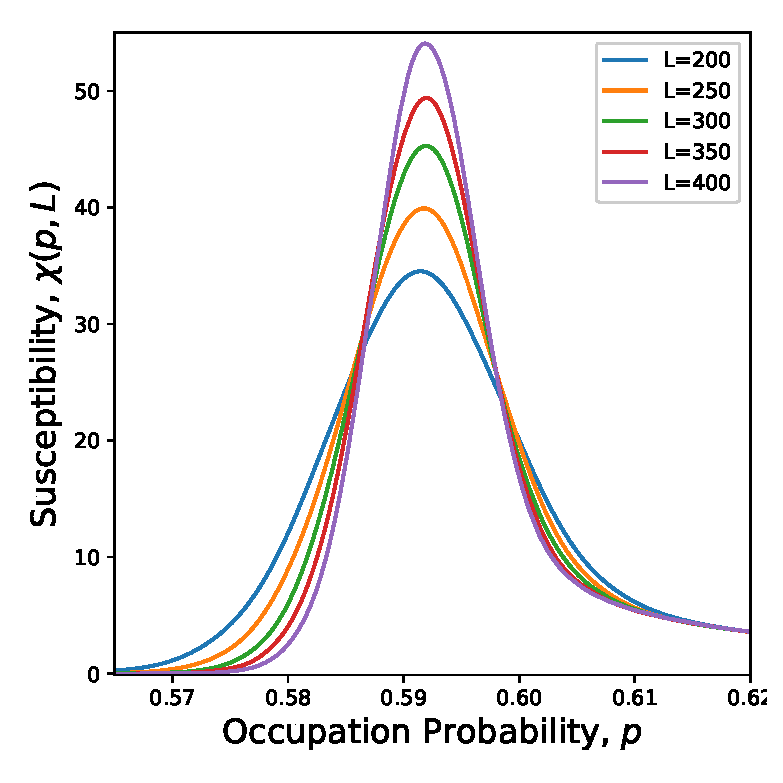
\includegraphics[width=\linewidth]{{{L0/sq_lattice_site_percolation_periodic__susceptibility-pc0.5927}}}
				\caption{L0}
			\end{subfigure}
			\begin{subfigure}{0.329\textwidth}
				\centering
				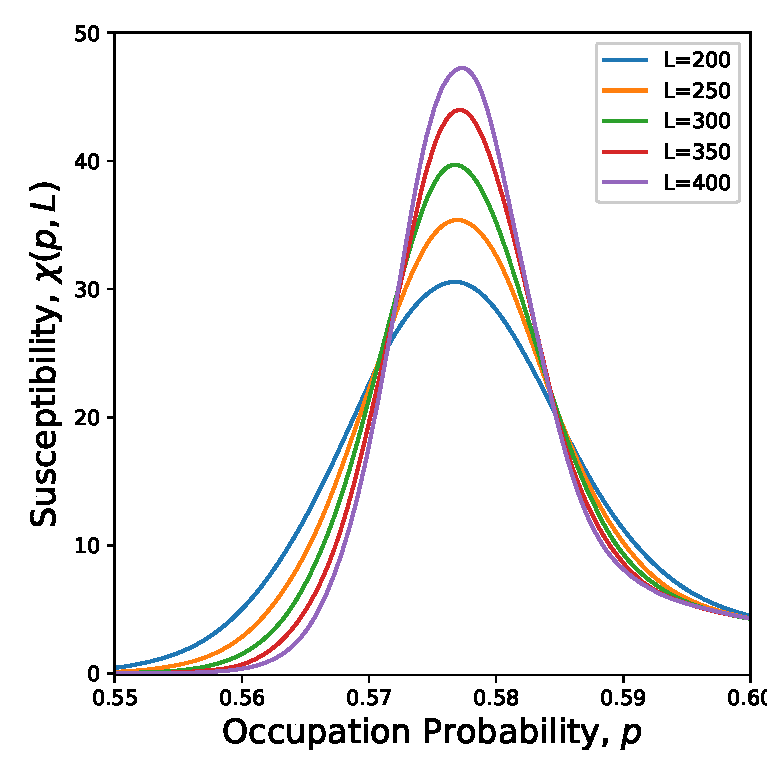
\includegraphics[width=\linewidth]{{{L1/sq_lattice_site_percolation_ballistic_deposition_L1_periodic__susceptibility-pc0.5782}}}
				\caption{L1}
			\end{subfigure}
			\begin{subfigure}{0.329\textwidth}
				\centering
				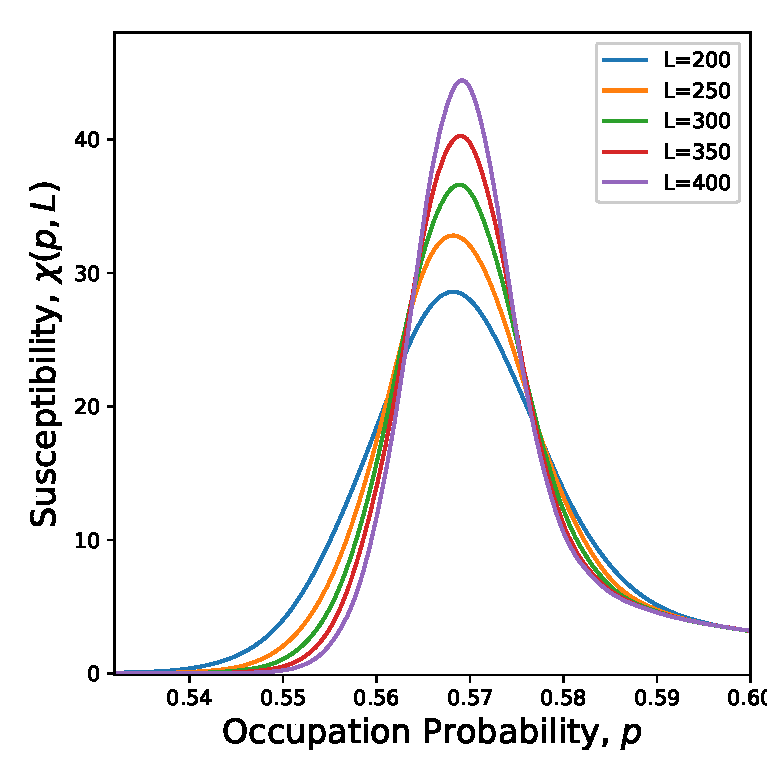
\includegraphics[width=\linewidth]{{{L2/sq_lattice_site_percolation_ballistic_deposition_L2_periodic__susceptibility-pc0.5701}}}
				\caption{L2}
			\end{subfigure}
			\caption{Susceptibility, $\chi(p,L)$ vs Occupation Probability, $p$}
			\label{fig:susceptibility}
		\end{figure}
		\begin{figure}
				\begin{subfigure}{0.329\textwidth}
				\centering
				\includegraphics[width=\linewidth]{{{sq_lattice_site_percolation_periodic__susceptibility-x-scaled-pc0.5927_gamma_0.6407_nu_0.750}}}
				\caption{L0}
			\end{subfigure}
			\begin{subfigure}{0.329\textwidth}
				\centering
				\includegraphics[width=\linewidth]{{{sq_lattice_site_percolation_ballistic_deposition_L1_periodic__susceptibility-x-scaled-pc0.5782_gamma_0.6287_nu_0.736}}}
				\caption{L1}
			\end{subfigure}
			\begin{subfigure}{0.329\textwidth}
				\centering
				\includegraphics[width=\linewidth]{{{sq_lattice_site_percolation_ballistic_deposition_L2_periodic__susceptibility-x-scaled-pc0.5701_gamma_0.6362_nu_0.721}}}
				\caption{L2}
			\end{subfigure}
			\caption{$\chi(p,L)$ vs $(p-p_c) L ^{1/\nu}$}
			\label{fig:susceptibility-x-scaled}
		\end{figure}
		\begin{figure}
			\begin{subfigure}{0.329\textwidth}
				\centering
				\includegraphics[width=\linewidth]{{{sq_lattice_site_percolation_periodic__susceptibility-data_collapse-pc0.5927_gamma_0.6407_nu_0.750}}}
				\caption{L0}
			\end{subfigure}
			\begin{subfigure}{0.329\textwidth}
				\centering
				\includegraphics[width=\linewidth]{{{sq_lattice_site_percolation_ballistic_deposition_L1_periodic__susceptibility-data_collapse-pc0.5782_gamma_0.6287_nu_0.736}}}
				\caption{L1}
			\end{subfigure}
			\begin{subfigure}{0.329\textwidth}
				\centering
				\includegraphics[width=\linewidth]{{{sq_lattice_site_percolation_ballistic_deposition_L2_periodic__susceptibility-data_collapse-pc0.5701_gamma_0.6362_nu_0.721}}}
				\caption{L2}
			\end{subfigure}
			\caption{$\chi L^{\gamma/\nu}$ vs $(p-p_c) L ^{1/\nu}$}
			\label{fig:susceptibility-data-collapse}
		\end{figure}
	\subsection{Cluster Size Distribution}
		\begin{figure}
			\caption{Number of cluster of size $s$, $n_s$ vs size of the cluster $s$}
		\end{figure}
		\begin{figure}
			\caption{$\log(n_s)$ vs $\log(s)$}
		\end{figure}
	$n_s$ vs $s$ graph
	\subsection{Cluster Rank Size Distribution}
	\subsection{Order-Disorder Transition}
	    Phase transition is an order-disorder transition. There is a critical point which separates the two regions. Before the critical point the system is in disordered phase and after it is in ordered phase when we increase temperature in thermodynamics. Behavior of two phases are completely different. It's astonishing how the behavior changes. In percolation theory, this order disorder transition is different than in thermodynamics. Here disordered means uncertainty, since we are dealing with a system where probability is the control parameter (the occupation probability $p$). When $p$ is minimum all clusters are disconnected and have size of unity. This means that we can to pick a cluster with probability $\frac{1}{2L^2}$, where $L$ is the lattice size and $2L^2$ is the number of bonds in the lattice. That's why entropy is maximum and order parameter is minimum in this region. Now as we keep occupying the lattice clusters of different size arises, and at some point a miracle happens. It is the critical point where the transition occurs. A cluster appears for the first time which spans the entire lattice either horizontally or vertically. And in case of periodic condition the cluster wraps the lattice all the way around it. This cluster is called the spanning (wrapping) cluster in non-periodic (periodic) condition. The probability of picking this cluster at random is always larger than picking any other clusters. Thus system goes to the ordered state. And if we keep occupying the lattice at some point all cluster are joined to form one cluster. Thus picking this cluster at random has no uncertainty, meaning we have reached the entirely ordered phase. Here entropy is minimum and ordered parameter is maximum. A graph \ref{fig:ordered-disordered-transition} containing both entropy and order parameter can show this process. We have normalized the entropy (figure \ref{fig:entropy}) to match with the order parameter (figure \ref{fig:order-parameter}).

		\begin{figure}
			\begin{subfigure}{0.329\textwidth}
				\centering
				\includegraphics[width=\linewidth]{{{sq_lattice_site_percolation_periodic__entropy_by_site-entropy-order_parameter-L400}}}
				\caption{L0}
			\end{subfigure}
			\begin{subfigure}{0.329\textwidth}
				\centering
				\includegraphics[width=\linewidth]{{{sq_lattice_site_percolation_ballistic_deposition_L1_periodic_-entropy-order_parameter-L400}}}
				\caption{L1}
			\end{subfigure}
			\begin{subfigure}{0.329\textwidth}
				\centering
				\includegraphics[width=\linewidth]{{{sq_lattice_site_percolation_ballistic_deposition_L2_periodic_-entropy-order_parameter-L400}}}
				\caption{L2}
			\end{subfigure}
			\label{fig:ordered-disordered-transition}
			\caption{$H(p,L)/H(0,L)$ or $P(p,L)/P(1,L)$ vs $p$}
		\end{figure}
	\subsection{Fractal Dimension}
		At critical point the square lattice shows the property of a fractal. A fractal is an object which occupies less space than it is embedded. For example a piece of cheese is a 3D fractal, since there are holes in the cheese which is empty. We use the relation
		\begin{equation}
			S \sim L^{d_f}
		\end{equation}
		taking $\log$ we get
		\begin{equation}
			\log(S) = d_f \log(L)
		\end{equation}
		Here $S$ is the average size of the spanning cluster at critical point. Using this we get the figure \ref{fig:fractal-dimension}. And we obtain fractal dimension $d_f$ for $L0,L1,L2$ which is listed in \ref{tab:exponents}. 
		\begin{figure}
			\begin{subfigure}{0.329\textwidth}
				\centering
				\includegraphics[width=\linewidth]{{{sq_lattice_site_percolation_periodic_-fractal_dimension_1.89394}}}
				\caption{L0}
			\end{subfigure}
			\begin{subfigure}{0.329\textwidth}
				\centering
				\includegraphics[width=\linewidth]{{{sq_lattice_site_percolation_ballistic_deposition_L1_periodic_-fractal_dimension_1.8995}}}
				\caption{L1}
			\end{subfigure}
			\begin{subfigure}{0.329\textwidth}
				\centering
				\includegraphics[width=\linewidth]{{{sq_lattice_site_percolation_ballistic_deposition_L2_periodic_-fractal_dimension_1.9081}}}
				\caption{L2}
			\end{subfigure}
			\label{fig:fractal-dimension}
			\caption{$\log(S)$ vs $\log(L)$}
		\end{figure}

